The presence of a magnetic field modifies the particle momentum, in particular $p_{x}$ and $p_{y}$, changing the entrance position and incidence angle to the dRICH. In addition, it may cause the particle to continue to change directory within the radiator volume, smearing out the Cerenkov ring. This effect needs to be checked in full simulations of the dRICH detector in the magnetic field to determine if corrector cois are required to shape the magnetic field. In this section we look at the impact of this effect on the performance of the dRICH detector. Figure~\ref{fig:drich_p4_xy} shows Cherenkov ring produce by 4~GeV electrons, pions, and kaons with and without magnetic field. 
\begin{figure}[h!tbp]
    \centering
    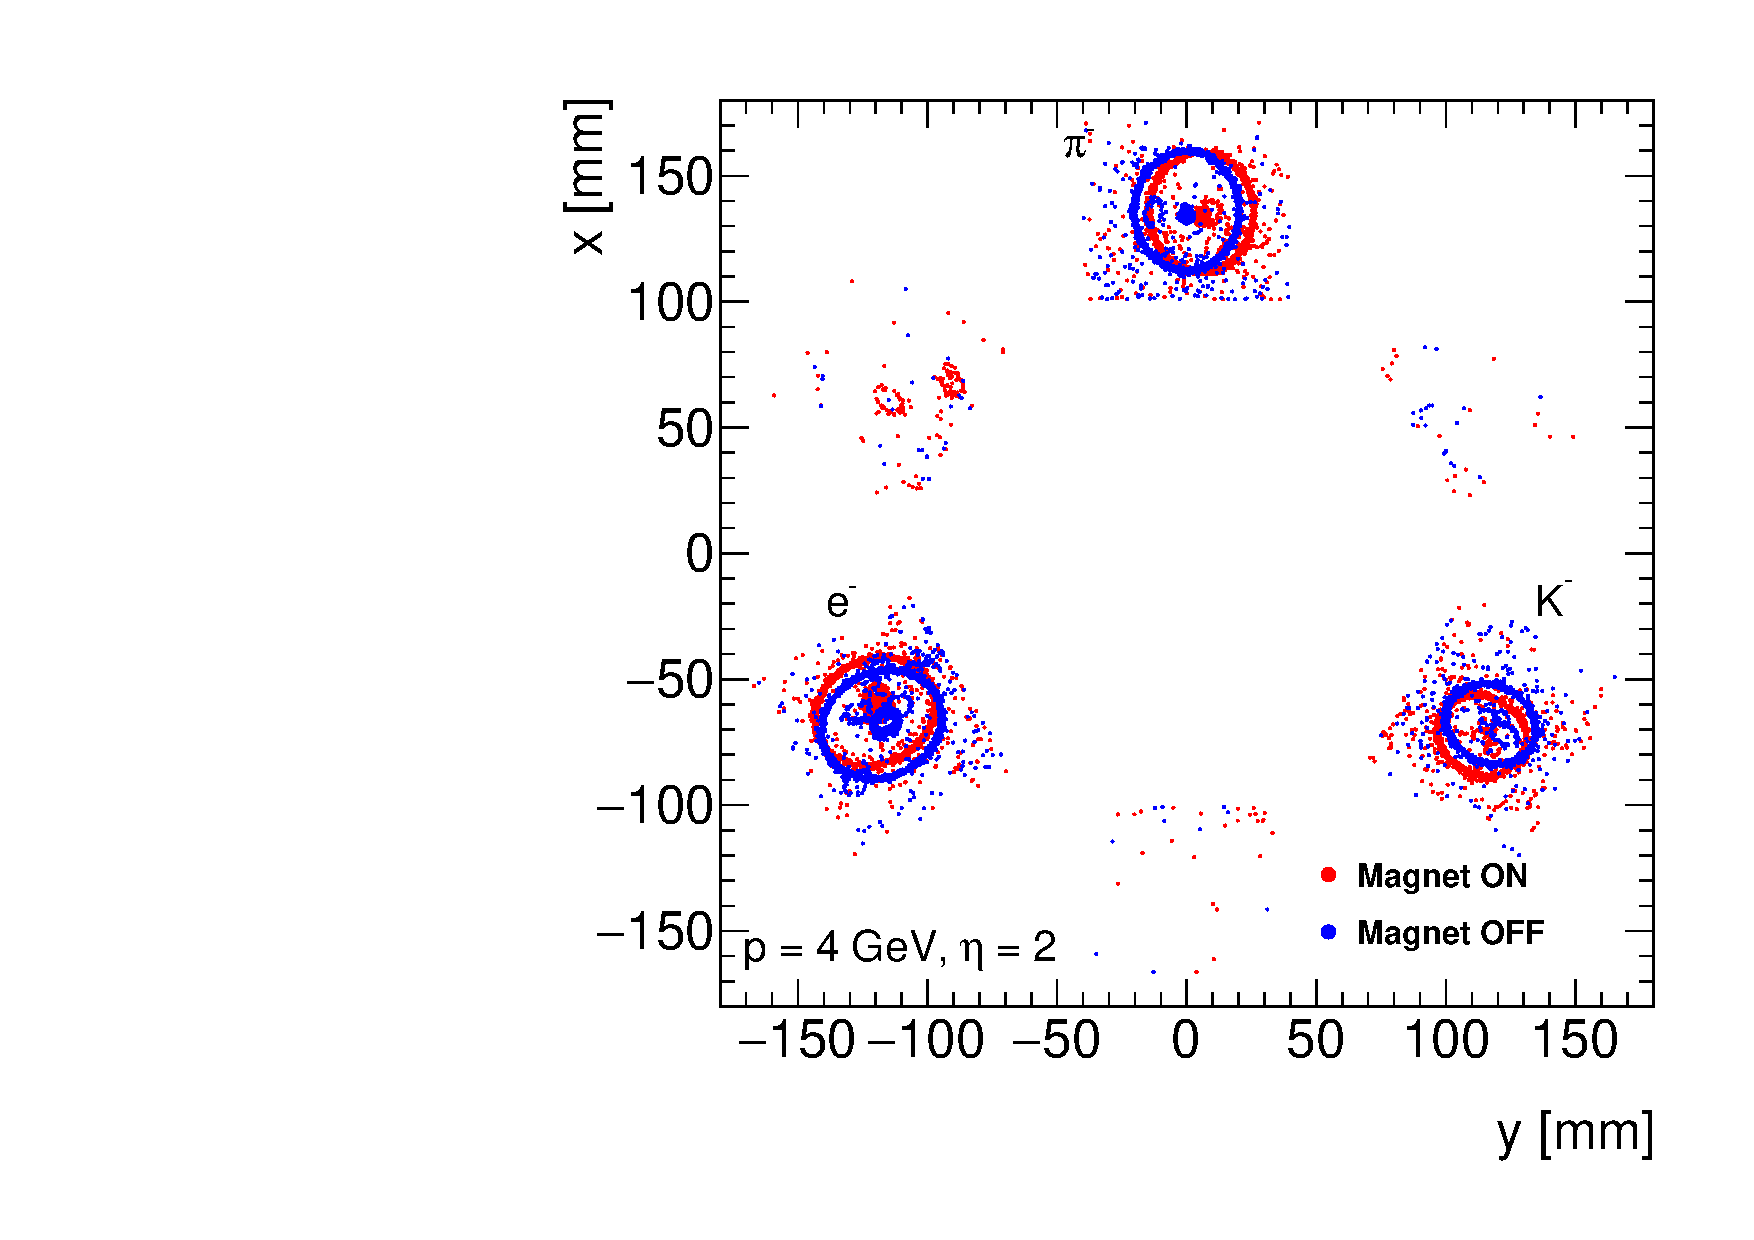
\includegraphics[width=0.5\textwidth]{figs/rings_xy_p4_fornote.pdf}
    \caption{dRICH hits, from events including 4~GeV electrons, pions, and kaons.}
    \label{fig:drich_p4_xy}
\end{figure}
To understand the impact of the magnetic field we look at the modification of the radius and width of the ring of electrons, pions, and kaons for three values of momentum, 1, 4, and 10~GeV. Figure~\ref{fig:drich_pX_e} shown dRICH hits centered at (0,0) in $(\eta,\phi)$ space with and without the magnetic field. We can see for 1~GeV electrons there is small smear of the inner (Gas) ring when the magnetic field is turned-on. 
\begin{figure}[h!tbp]
    \centering
    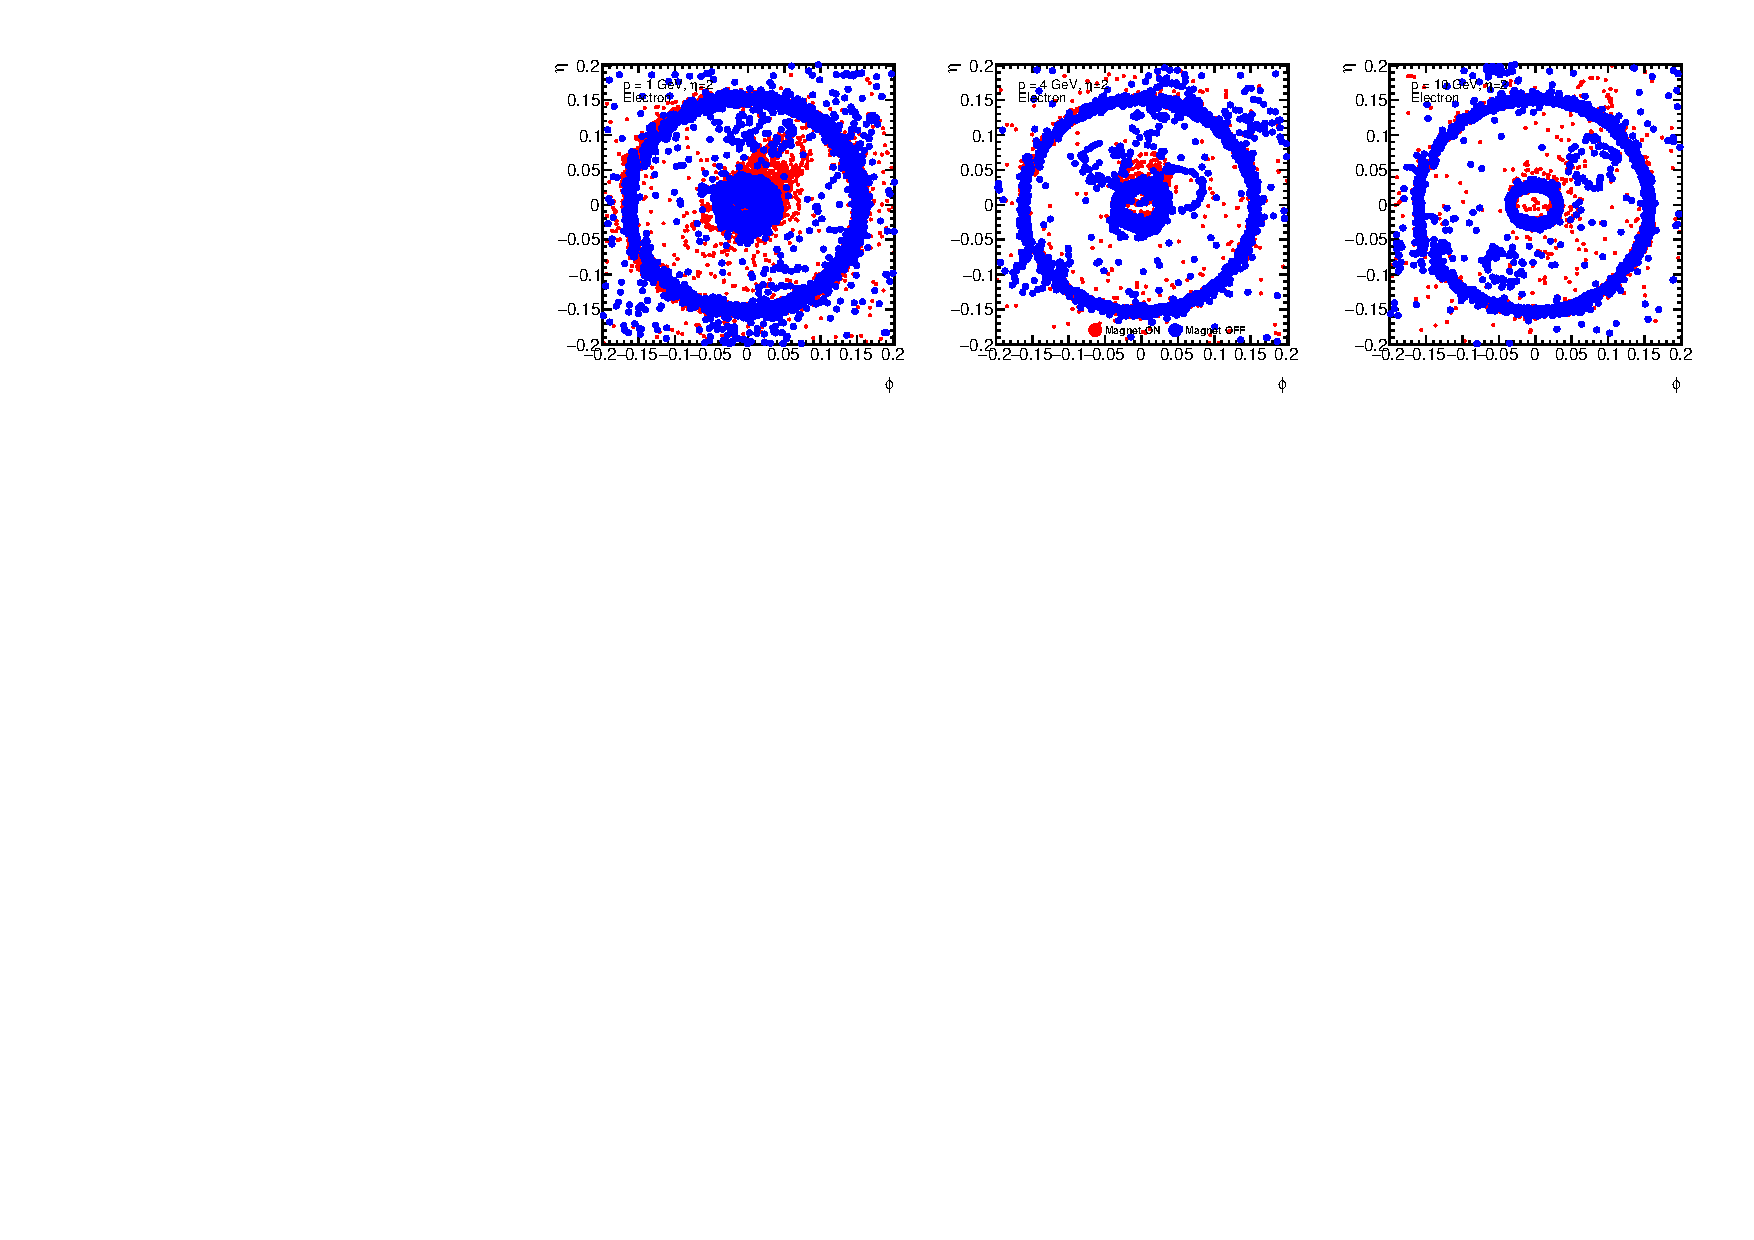
\includegraphics[width=0.9\textwidth]{figs/rings_etaphi_electron.pdf}
    \caption{dRICH hits for 1, 4 and 10~GeV electron events. The ring centers have been overlaid to allow a direct comparison without magnetic field (blue) and with the magnetic field on (red). }
    \label{fig:drich_pX_e}
\end{figure}
The radius distribution is calculated as $R=\sqrt{\phi^{2}+\eta^{2}}$ for each dRICH hit, we can compare this with magnetic field turned-on and off. In Figure~\ref{fig:drich_radius_p1_ePiK} we can see a small tail in the radius distribution for Gas ring of low p electrons. This small modification in the radius width is not expected to cause a degradation in the PID performance.
\begin{figure}[h!tbp]
    \centering
    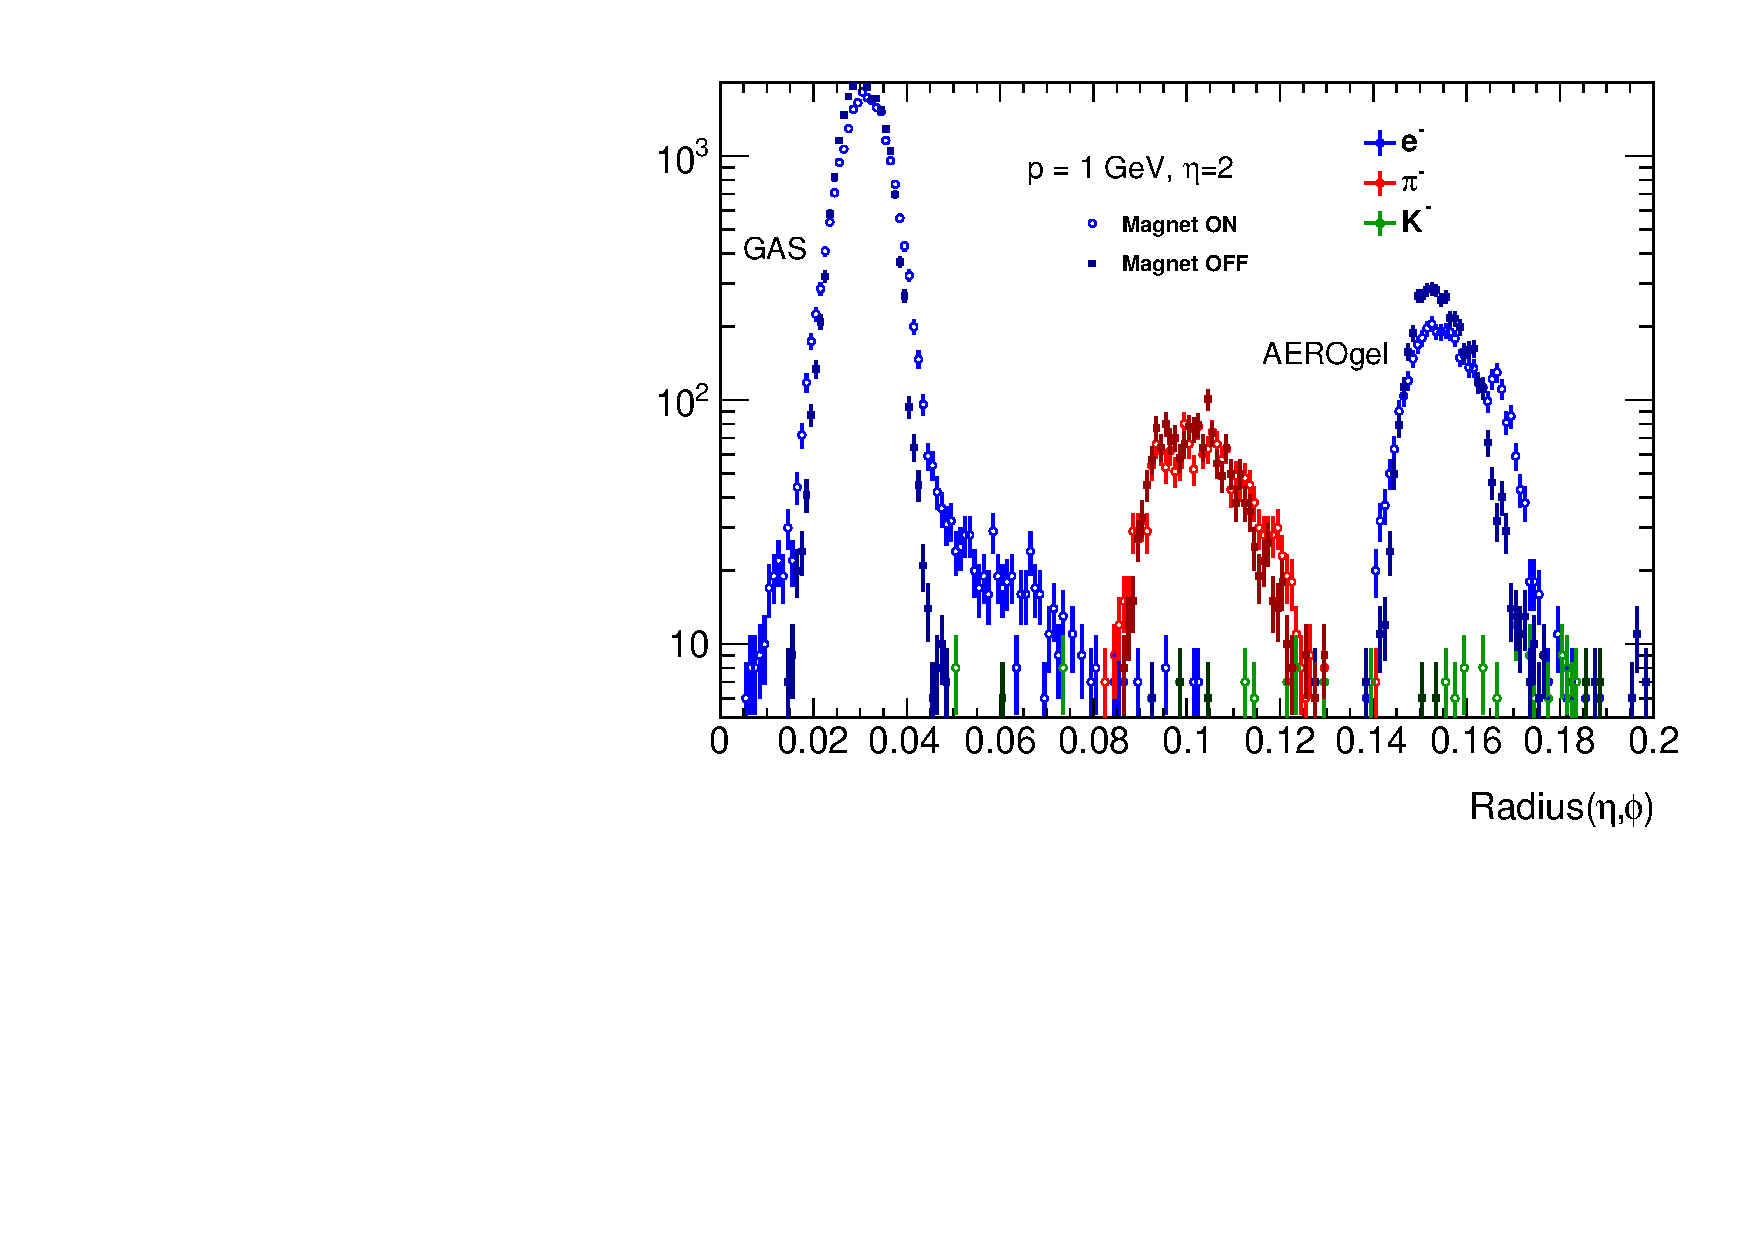
\includegraphics[width=0.7\textwidth]{figs/Radius_p1_shift.pdf}
    \caption{Distribution of the Cereknov ring radius distribution of 1~GeV electrons, pion and kaons, with the magnetic field on and off.  With the magnetic field on a slight smearing of the electron ring distribution can be observed. }
    \label{fig:drich_radius_p1_ePiK}
\end{figure}